%%% Lecture 7

\section{Hopf Fibration}

\lecture[We construct the thing on the background of Schwede's homepage (Hopf fibration) and we introduce the long exact sequence associated to a fiber bundle (we also use our new toys to compute $\pi_3(S^2)$).]{2021-11-8}

The goals of the following two lectures (which are given by Markus Hausmann, a PhD student of Schwede) are:
\begin{enumerate}
    \item to construct the \textbf{Hopf fibration}, a fibre bundle $\eta:S^3\to S^2$ with fibre $S^1$,
    \item to associate to every fibre bundle $p:E\to B$ a long exact sequence of the form
    \[\cdots\to\pi_n(p^{-1}(b),e)\xto{i_*}\pi_n(E,e)\xto{p_*}\pi_n(B,b)\to\pi_\ni(p^{-1}(b),e)\to\cdots\]
\end{enumerate}

When we are done, we will have as a corollary the computation of our first \textit{really} non-trivial homotopy group.

\begin{corollary}
For every $n\geq 3$ there is an isomorphism $\pi_n(S^3,*)\cong\pi_n(S^2,*)$. In particular, $\pi_3(S^2,*)\cong\Z$, generated by the class of the Hopf fibration.
\end{corollary}

\begin{proof}
For $n\geq3$ we have
\[\cdots\to\pi_n(S^1,*)=0\to\pi_n(S^3,*)\xto{\eta_*}\pi_n(S^2,*)\to\pi_\ni(S^1,*)=0\to\cdots\]
which yields the claim.

In particular, for $n=3$ we get that $\eta_*:\pi_3(S^3,*)\cong\Z\to\pi_3(S^2,*)$ is an isomorphism which sends $[\id_{S^3}]$, generator of $\pi_3(S^3,*)$, to $[\eta\circ\id_{S^3}]=[\eta]$.
\end{proof}

The Hopf fibration is part of a family of fibre bundles.

Let $K=\R$ or $\CC$ and recall the projective spaces:
\[\kpn=(K^{n+1}\sm\cb{0})/K^\times\]
where $x\sim\lambda x$ for all $x,\lambda\in K^\times$. In particular, we have that:
\begin{enumerate}[label={-}]
    \item $\rpn$ is an $n$-dimensional manifold,
    \item $\cpn$ is a $2n$-dimensional manifold.
\end{enumerate}
Moreover, recall that $\rp{1}\cong S^1$ and $\cp{1}\cong S^2$.

We consider now the projections $p:K^{n+1}\sm\cb{0}\to\kpn$.

Let $G$ be a topological group. A principal $G$-bundle is a $G$-space $E$ such that:
\begin{numerate}
    \item for every $e\in E$ the map $G\to Ge=\cb{ge\mid g\in G}$, $g\to ge$, is a homeomorphism,
    \item the quotient map $p:E\to E/G=E/\sim$, where $e\sim ge$ for all $e\in E$, $g\in G$, is a fibre bundle.
\end{numerate}

\begin{example}
The group action of the additive group of the real numbers with the discrete topology on itself (with the standard topology):
\[\R^d\times\R\to\R\]
is an example of free action which does not satisfy property (2).\todo{Not sure}
\end{example}

\begin{proposition}
 For $K=\R$ or $\CC$, the $K^\times$ action on $K^{n+1}\sm\cb{0}$ is a $K^\times$-principal bundle.
\end{proposition}

\begin{proof}
Let $e\in K^{n+1}\sm\cb{0}$. Then the map
\[K^\times\to K^\times e,\ \ \lambda\mapsto\lambda e\]
is continuous and satisfies $\|\lambda_1 e-\lambda_2 e\|=|\lambda_1-\lambda_2|\|e\|$. It follows that the inverse is also continuous.

It remains to show that $K^{n+1}\sm\cb{0}\to \kpn$ is a locally trivial fibre bundle. For $1\leq i\leq n+1$ let $X_i\subset K^{n+1}\sm\cb{0}$ be the subspace of tuples $(x_1,\dots,x_{n+1})$ such that $x_i\neq 0$, i.e. $x_i\in K^\times$. Then $K^{n+1}\sm\cb{0}=\cup_{i=1}^{n+1}X_i$. Let $Y_i=p(X_i)\subset \kpn$. This is open since $p^{-1}(Y_i)=X_i$. We define $u:p^{-1}(Y_i)=X_i\to Y_i\times K^\times$ by $u(x)=(p(x),x_i)$, with inverse
\[u^{-1}([x],\lambda)=(x_1/x_i,\dots,x_{i-1}/x_i,\lambda,x_{i+1}/x_i,\dots,x_{n+1}/x_i).\]
\end{proof}

For $K=\CC$ and $n=1$ this gives a fibre bundle
\[p:\CC^2\sm\cb{0}\cong S^3\to \cp{1}\cong S^2\]
with fibre $\CC^\times\cong S^1$. This is already the Hopf fibration "up to homotopy".

Let $S(K^n)\subset K^n$ be the unit sphere ($(n-1)$-dimensional if $K=\R$, $(2n-1)$-dimensional if $K=\CC$). Further, let $G(K)\subset K^\times$ be the subgroup of elements of norm $1$ ($G(\R)=\cb{\pm1}$, $G(\CC)=S^1$). Then the $K^\times$-action on $K^{n+1}\sm\cb{0}$ restricts to a $G(K)$-action on $S(K^{n+1})$ and the induced map
\begin{center}
    \begin{tikzcd}
    S(K^{n+1})\arrow[r]\arrow[dr] & K^{n+1}\sm\cb{0}\arrow[r] & \kpn \\
    & S(K^{n+1})/G(K)\arrow[ur,swap,"\cong"]
    \end{tikzcd}
\end{center}
is a homeomorphism.

\begin{proposition}
The $G(K)$-action on $S(K^{n+1})$ defines a $G(K)$-principal bundle with base space $\kpn$.
\end{proposition}

\begin{proof}
Let $X_i\subset K^{n+1}\sm\cb{0}$, $Y_i\subset \kpn$ as before. We obtain a homeomorphism
\[v:q^{-1}(Y_i)=S(K^{n+1})\cap X_i\to Y_i\times G(K),\ \ x\mapsto (q(x),x_i/|x_i|).\]
\end{proof}

For $K=\R$ we obtain the covering space $S^n\to\rpn$ we already knew.

For $K=\CC$ we get a fibre bundle $S^{2n+1}\to\cpn$ with fibre $S^1$. For $n=1$ we get the Hopf fibration $\eta:S^3\to S^2$.

\begin{remark}
The Hopf fibration decomposes $S^3$ as a disjoint union of circles, continuously indexed over $S^2$.
It can be shown that any two of them are linked!

Considering $\eta:S^3\to S^2$ and $x_1\neq x_2\in S^2$
\[s:S^3\supset\eta^{-1}(x_1)\times\eta^{-1}(x_2)\to S^2,\ (x,y)\to\frac{x-y}{||x-y||}\]
is continuous. Choosing orientations on $S^2$ and $\eta^{-1}(x_1)\times\eta^{-1}(x_2)\cong S^1\times S^1$, we can consider the mapping degree of $s$. This is an example of an invariant for links called the \textbf{linking number} and it will be $\pm1$ in this case.
\end{remark}\smallskip

%\rightnote{Xiaoxiang Zhou suggested \href{https://www.youtube.com/watch?v=yNpqLMpfxA8&list=PL3C690048E1531DC7&index=7}{Dimension: a walk through mathematics} for an animation of the Hopf fibration.}

\begin{center}\rightnote{Someday I'll really wrap my head around this picture... (but maybe it's just not \textit{that} illuminating?)}
    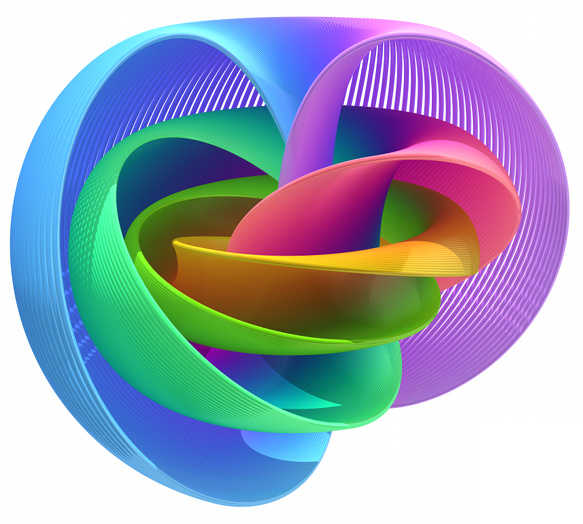
\includegraphics[scale=0.45]{Pictures/HopfFibration.jpg}
\end{center}

\section{The Long Exact Sequence Associated to a Serre Fibration}

We turn now to our second goal. If $p:E\to B$ is a fibre sequence, $b\in B$, $e\in p^{-1}(b)$, then we want to show that there is a long exact sequence of the form:
\[\cdots\to\pi_n(p^{-1}(b),e)\to\pi_n(E,e)\to\pi_n(B,b)\to\cdots\]

\begin{example}
Let $p:E\to B$ be a covering space. We get a long exact sequence (assuming $E$ is connected):
\[\cdots\to\pi_n(p^{-1}(b),e)=0\to\pi_n(E,e)\to\pi_n(B,b)\to\pi_\ni(p^{-1}(b),e)=0\to\cdots\]
\[\cdots\to 0 \to\pi_1(E,e)\to\pi_1(B,b)\to\pi_0(p^{-1}(b),e)\to 0\]

This amounts to the known statements that $p_*:\pi_1(E,e)\to\pi_1(B,b)$ is injective (and that the fiber can be identified, via path lifting, with the set of cosets of $p_*\pi_n(E,e)$ in $\pi_1(B,b)$) and that $p_*:\pi_n(E,e)\to\pi_n(B,b)$ is an isomorphism for $n\geq 2$. Both facts have been already proven using the lifting properties of covering spaces.\rightnote{He adds a reminder on map lifting here.}
\end{example}

Let $p:E\to B$ be a continuous map. A \textbf{test situation} for the homotopy lifting property (HLP) consists of a space $X$ and a commutative square:
\begin{center}
    \begin{tikzcd}
    X \arrow[d,"i_0"] \arrow[r,"f"] & E \arrow[d,"p"] \\
    X\times[0,1] \arrow[r,"H"] & B
    \end{tikzcd}
\end{center}

A solution to the test situation is a map $\til H:X\times[0,1]\to E$
 such that $p\circ\til H=H$ and $\til H\circ i_0=f$.
 
 there is also a relative version: a pair of spaces $\pairs$ and a commutative diagram:
\begin{center}
    \begin{tikzcd}
    X\times\cb{0}\cup(A\times[0,1]) \arrow[d, hook,"i_0"] \arrow[r,"f"] & E \arrow[d,"p"] \\
    X\times[0,1] \arrow[r,"H"] & B
    \end{tikzcd}
\end{center}

A solution is again a map $\til H:X\times[0,1]\to E$ such that $p\circ\til H=H$ and $\til H\circ i_0=f$.

A map $p:E\to B$ is called a \textbf{Hurewicz fibration} if it has the HLP with respect to all $X$ and all absolute test-situations for $X$.

A map $p:E\to B$ is called a \textbf{Serre fibration} if it has the HLP with respect to every CW-complex $X$ and all absolute test-situations for $X$.

For the proof of the existence of the long exact sequence associated to a fibre bundle we need two intermediate results.

\begin{proposition**}
Let $p:E\to B$ be a Serre fibration, $Y\subset B$ a subspace and $x\in p^{-1}(Y)$. Then the projection induces an isomorphism (for $n\geq 1$):
\[p_*:\pi_n(E,p^{-1}(Y),x)\xto{\cong}\pi_n(B,Y,p(x))\]
\end{proposition**}

\begin{corollary**}
Let $Y=\cb{b}$. We get a long exact sequence:
\[\cdots\to\pi_n(p^{-1}(b),x)\to\pi_n(E,x)\to\pi_n(E,p^{-1}(b),x)\cong\pi_n(B,b)\to\cdots\]
\end{corollary**}

\begin{theorem**}
Every fiber bundle is a Serre fibration.
\end{theorem**}
